% Chapter Template

\chapter{Quadratic Programming} % Main chapter title

\label{ChapterX} % Change X to a consecutive number; for referencing this chapter elsewhere, use \ref{ChapterX}

%----------------------------------------------------------------------------------------
%	SECTION 1
%----------------------------------------------------------------------------------------
An optimisation problem with a quadratic objective function and linear constraints is called a quadratic program. Problem of this type are important in their own right, and they also arise as subproblems in methods for general constrained optimisations. 

\section{Definition of QP}

The general quadratic program(QP) can be stated as

\begin{equation}
\begin{aligned}
& \underset{x}{\text{min}}
& & q(x)= \frac{1}{2}x^{T}Gx+x^{T}c \\
& \text{subject to} & &  a_{i}^{T}x = b_i & i\in \mathbb{E} \\
& & &  a_i^{T}x \geqslant b_{i} & i\in \mathbb{I}
\end{aligned}
\label{eqn:quadratic_programming}
\end{equation}
where $G$ is a symmetric $n\times n$ matrix, $E$ and $I$ are finite sets of indices, and $c$,$x$, and $a_i, i\in E \cup I$, are vectors in $\mathbb{R}^n$. Quadratic programs can always be solved (or shown to be infeasible) in a finite amount of computation, but the effort required to find a solution depends strongly on the characteristics of the objective function and the number of inequality constraints. If the Hessian matrix $G$ is positive semidefinite, we say that \ref{eqn:quadratic_programming} is a convex QP, and in this case the problem is often similar in difficulty to a linear program. (Strictly convex QPs are those in which G is positive definite.) Nonconvex QPs, in which G is an indefinite matrix, can be more challenging because they can have several stationary points and local minima.

In this chapter we will try to show different kinds of quadratic programs but we will mainly focus on convex quadratic program and different algorithms of convex quadratic programs.

\section{Classification of QP's}

Some classification of quadratic program's:
\begin{itemize}
	\item Unconstrianed QP
	\item Box constrained QP
	\item Equality constrained QP
	\item Inequality constrained QP.
\end{itemize}

\section*{Important Definitions}
\subsection*{Logarithmic barrier}
Consider inequalities $Ax \leqslant b$ with $A$ of size $m\times n$ and with rows $a_i^T$. Define
\begin{equation*}
P=\lbrace x \mid Ax \leqslant b \rbrace \text{ and } P^0=\lbrace x \mid Ax < b \rbrace
\end{equation*}
logarithmic barrier for the inequalities $Ax\leqslant b$:
\begin{equation*}
\begin{aligned}
	\phi(x) = - \sum_{i=1}^{m}\log(b_i - a_i^Tx) & & \text{with domain } P^0
\end{aligned}	
\end{equation*}
\begin{figure}[h]
\centering
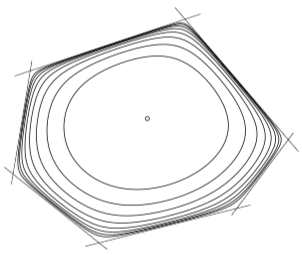
\includegraphics[scale=0.5]{Figures/logarithmic_barrier.png}
\decoRule
\caption[hypercube]{Logarithmic barrier function.}
\label{fig:logarithmic_barrier}
\end{figure}


\subsection*{Gradient}
Gradient $\nabla \phi(x)$ is the n-vector with $\nabla \phi(x)_i = \frac{\delta \phi (x)}{\delta x_i}$
\begin{equation*}
	\begin{aligned}
		\nabla \phi(x) = \sum_{k=1}^{m} \frac{1}{b_k-a_k^Tx}a_k = A^Td_x 
	\end{aligned}
\end{equation*}
$d_x$ denotes the positive $m-$vector
\begin{equation*}
	\begin{aligned}
		d_x = \left( \frac{1}{b_1-a_1^Tx},..., \frac{1}{b_m-a_m^Tx} \right)
	\end{aligned}
\end{equation*}


\subsection*{KKT System}
KKT System is

\subsection*{Hessian Matrix}
Hessian Matrix Gradient $\nabla^2 \phi(x)$ is the $n\times n$-matrix with $\nabla \phi (x)_{ij} = \frac{\delta^2 \phi (x)}{\delta x_i \delta x_j}$

\begin{equation*}
	\begin{aligned}
		\nabla^2 \phi(x) = \sum_{k=1}^{m} \frac{1}{(b_k-a_k^Tx)^2} a_k a_k^T = A^T diag(d_x)^2 A 
	\end{aligned}
\end{equation*}

\subsection*{Central Path}
Consider the linear programming problem in standard form:
\begin{equation*}
\begin{aligned}
\text{min } c^Tx, & & \text{subject to} Ax=b, \geqslant 0	
\end{aligned}
\end{equation*}
where $c$ and $x$ are vectors in $\mathbb{R}^n$, b is a vector in $\mathbb{R}^m$, and $A$ is an $m\times n$ matrix with full row rank. The dual problem of the above problem is
\begin{equation*}
\begin{aligned}
	\text{max } b^T\lambda, & & \text{subject to} A^T\lambda + s = c, x\geqslant 0
\end{aligned}
\end{equation*}
where $\lambda$ is a vector in $\mathbb{R}^m$ and s is a vector in $\mathbb{R}^n$
The primal-dual feasible set $\mathcal{F}$ and strictly feasible set $\mathcal{F}^0$ are defined as
\begin{equation*}
	\begin{aligned}
		\mathcal{F} &= \lbrace (x,\lambda,s) \mid Ax=b, A^T\lambda +s = c, (x,s) \geqslant0 \rbrace\\
		\mathcal{F}^0 &= \lbrace (x,\lambda,s) \mid Ax=b, A^T\lambda +s = c, (x,s) > 0 \rbrace
	\end{aligned}
\end{equation*}
The central path $C$ is an arc of strictly feasible points. It is parameterized by a scalar $\eta > 0$, and each point $(x_\tau ,\lambda_\tau, s_\tau)\in \mathcal{C}$ satisfies the following equations:
\begin{equation*}
	\begin{aligned}
		A^T\lambda+s &= c,\\
		Ax &= b,
		x_i,s_i &= \tau & & i = 1,2,...n.\\ 
		(x,s ) & > 0.
	\end{aligned}
\end{equation*}
So the central path is defined as:
\begin{equation*}
\begin{aligned}
	\mathcal{C} = \lbrace (x_\tau,\lambda_\tau, s_\tau)\mid \tau>0\rbrace
\end{aligned}
\end{equation*}
Another way of defining $\mathcal{C}$ is:
\begin{equation*}
\begin{aligned}
F(x_\tau,\lambda_\tau, s_\tau)=
	\begin{bmatrix}
		0\\
		0\\
		\tau e
	\end{bmatrix},
	(x_\tau,s_\tau) > 0
\end{aligned}
\end{equation*}

the conditions approximate more and more colsely as $\tau$ goes to zero. If $\mathcal{C}$ converges to anything as $\tau \downarrow 0$, it must converge to a primal-dual solution of the linear program.


\subsection*{Active set}
The Active set $\mathbb{A}(x)$ at any feasible $x$ consists of the equality constraint indices from $\varepsilon$ together with the indices of the inequality constraints $i$ for which $c_i(x)=0$; that is,
\begin{equation*}
	\begin{aligned}
		\mathbb{A}(x)=\varepsilon \cup {i\in \mathbb{I}\mid c_i(x)=0}
	\end{aligned}
\end{equation*}
At a feasible point x, the inequality constraint $i\in \mathbb{I}$ is said to be active if $c_i(x)=0$ and inactive if the strict inequality $c_i(x)>0$ is satisfied.

\section{Equality-Constrained Quadratic Programs}

We start this section with of algorithms for quadratic programming by considering the case of equality constrained

\subsection*{Properties of Equality-constrained QPs}
To make it simple, we write the equality constraint in a form of matrix and define it as follows:

\begin{equation}
\begin{aligned}
& \underset{x}{\text{min}}
& & q(x)= \frac{1}{2}x^{T}Gx+x^{T}c \\
& \text{subject to} & &  Ax=b
\end{aligned}
\label{eqn:equality_constrained_QP}
\end{equation}

where $A$ is the $m\times n$ Jacobian of constraints (with $m\leqslant n$) whose rows are $a_i^T,i \in \mathbb{E}$ and $b$ is the vecotor in $\mathbb{R}^n$ whose componants are $b_i, i \in \mathbb{E}$. Currently, we consider that $A$ has a full row rank (rank m) so that the constraints are consistent.

The first-order necessary conditions for $x^*$ to be a solution of \ref{eqn:equality_constrained_QP} state that there is a vector $\lambda^*$ such that the following system of equations is satisfied:

\begin{equation}
\begin{bmatrix}
  	G & -A^T \\
    A & 0
  \end{bmatrix}
  \begin{bmatrix}
  	x^* \\
    \lambda{*}
  \end{bmatrix}
  =
  \begin{bmatrix}
  	-c \\
    b
  \end{bmatrix}	
  \label{eqn:Properties_of_EC_QP}
\end{equation}

These conditions are a consequence of the general result for first-order optimality conditions.  $\lambda^*$ is called the vector of Lagrange multipliers. In \ref{eqn:Properties_of_EC_QP} we can write $x^*$ as $x^* = x+p$ which makes it useful for computation, where x is some estimate of the solution and p is the desired step. By introducing this and rearranging the equations, we obtain

\begin{equation}
\begin{bmatrix}
  	G & A^T \\
    A & 0
  \end{bmatrix}
  \begin{bmatrix}
  	-p \\
    \lambda{*}
  \end{bmatrix}
  =
  \begin{bmatrix}
  	g \\
    h
  \end{bmatrix}	
  \label{eqn:Properties_of_EC_QP_2}
\end{equation}
where
\begin{equation}
\begin{aligned}
h= Ax-b, & g = c+Gx, & p = x^* - x.
\end{aligned}
\label{eqn:Properties_of_EC_QP_3}	
\end{equation}

The matrix \ref{eqn:Properties_of_EC_QP_2} is called the Karush-Kuhn-Tucker (KKT) matrix, and the following result gives conditions under which it is nonsingular. We will use $Z$ to denote the $n \times (n-m)$ matrix whose columns are basis for the null space of $A$. That is, $z$ has full  rank and satisfies $AZ=0$.

\begin{mybox}{Lemma}
\begin{lemma}
\textit{Let $A$ have full row rank, and assume that the reduce Hessian matrix $Z^TGZ$ is positive definite. Then the KKT matrix}

\begin{equation}
	\begin{bmatrix}
  		G & A^T \\
    	A & 0
    \end{bmatrix}
\label{eqn:Properties_of_EC_QP_4}	
\end{equation}
\textit{is nonsingular, and hence there is a unique vector pair $(x^*, \lambda^*)$ satisfying \ref{eqn:Properties_of_EC_QP}}.	
\label{lemma:KKT_nonsingularuty}
\end{lemma}
\end{mybox}

So, when the conditions of the \ref{lemma:KKT_nonsingularuty} is satisfied, there is a unique vector pair $(x^*, \lambda^*)$ that satiesfies the first-order necessary condition for \ref{eqn:equality_constrained_QP}. In fact, the second order sufficient conditions are also satisfied at $(x^*, \lambda^*)$, so $x^*$ is a strict local minimizer of \ref{eqn:equality_constrained_QP}. In fact we can use a direct argument to show that $x^*$ is a global solution of \ref{eqn:equality_constrained_QP}.

\begin{mybox}{Theorem}
\begin{theorem}
	Let A have full row rank and assume that the reduced-Hessian matrix $Z^TGZ$ is positive definite. Then the vector $x^*$ satisfying \ref{eqn:Properties_of_EC_QP} is the unique global solution of \ref{eqn:equality_constrained_QP}.
\end{theorem}
\end{mybox}
\begin{proof}
	Let x be any other feasible point (satisfying $Ax=b$), and as before, let $p$ denote the difference $x^*-x$. Since $Ax^*=Ax=b$, we have that $Ap=0$. By substituting into the objective function \ref{eqn:equality_constrained_QP}, we get
	\begin{equation}
	\begin{aligned}
		q(x) & = \frac{1}{2}(x^*-p)^TG(x^*-p)+C^T(x^*-p)\\
		& = \frac{1}{2}p^TGp-p^TGx^*-C^Tp+q(x^*)
	\end{aligned}
	\label{eqn:Properties_of_EC_QP_5}
	\end{equation}
	From \ref{eqn:Properties_of_EC_QP} we have that $Gx^*=-c+A^T\lambda^*$, so from $Ap = 0$ we have that
	\begin{equation}
	\begin{aligned}
		p^TGx^* &= p^T(-c)+A^T\lambda^* = -p^Tc.
	\end{aligned}
	\label{eqn:Properties_of_EC_QP_6}
	\end{equation}
	By substituting this relation into \ref{eqn:Properties_of_EC_QP_5}, we obtain
	\begin{equation}
	\begin{aligned}
		q(x)= \frac{1}{2} p^TGp + q(x^*).
	\end{aligned}
	\label{eqn:Properties_of_EC_QP_7}
	\end{equation}
	Since $p$ lies in the null space of $A$, we can write $p=Zu$ for some vector $u\in \mathbb{R}^{n-m}$, so that
	\begin{equation}
	\begin{aligned}
		q(x)= \frac{1}{2} u^TZ^TGZu + q(x^*).
	\end{aligned}
	\label{eqn:Properties_of_EC_QP_8}
	\end{equation}
	By positive definiteness of $Z^TGZ$, we conclude that $q(x)>q(x^*)$ except when $u=0$, that is, when $x=x*$. Therefore, $x^*$ is the unique global solution of \ref{eqn:equality_constrained_QP}
\end{proof}

When the reduced Hessian matrix $Z^TGZ$ is positive semidefinite with zero eigenvalues, the vector $x^*$ satisfying \ref{eqn:Properties_of_EC_QP_2} is a local minimizer but not a strict local minimizer. If the reduced Hessian has negative eigenvalues, then $x^*$ is only a stationary point, not a local minimizer.

\section{Direct Solution of the KKT System}

In this section we discuss the efficient methods of solving KKT system. The KKT system is always indefinite if $m\geqslant1$. We can apply direct techniques to solve indefinite KKT system.

\subsection*{Factoring the Full Scale System}
One option for solving KKT system is to perform triangular factorization on the full KKT matrix and then perform backward and forward substitution with the triangular factors. It is not possible to apply Cholesky factorization as it is indefinite.Another option can be Gaussian Elimination to obtain the $L$ and $U$ factors, but this method does not consider the symmetry.

So, the most effective strategy is to use symmetric indefinite factorization which has the form of:

\begin{equation}
	\begin{aligned}
		P^TKP = LDL^T
	\end{aligned}
	\label{eqn:SIF_1}
\end{equation}
where $P$ is an appropriately chosen permutation matrix. $L$ is lower triangular with $diag(L) = I$ and $D$ is block diagonal.
Based on \ref{eqn:SIF_1}, the KKT system \ref{eqn:Properties_of_EC_QP_2} is solved as follows:
\begin{equation}
	\begin{aligned}
		solve & & Ly = P^T
		\begin{bmatrix}
  		g \\
    	h
    \end{bmatrix}\\
    solve & & D\hat{y} = y\\
    solve & & L^T\bar{y} = \hat{y}\\
    set & & \begin{bmatrix}
  		-p \\
    	\lambda^*
    \end{bmatrix} = P\bar{y}
	\end{aligned}
	\label{eqn:SIF_2}
\end{equation}

This approach of factoring  the full $(n+m)\times (n+m)$ KKt matrix is quite effective  on many problems. It can be expensive when the permutation matrix $P$ are not able to maintain sparsity in the $L$ factor.
\subsection*{Range-space approach}
The range-space approach is useful when $G\in \mathbb{R}^{n\times n}$ is symmetric positive definite. We can multiply the first part of the equation \ref{eqn:Properties_of_EC_QP_2}  by $AG^-1$ and then subtract the second part to obtain a linear system in the vector $\lambda^*$ alone:

\begin{equation}
	\begin{aligned}
		(AG^{-1}A^T\lambda^*) = (AG^{-1}g-h)
	\end{aligned}
	\label{eqn:Range_space_1}
\end{equation}

We solve this symmetric semidifinite system for $\lambda^*$ and then recover $p$ from the first equation in \ref{eqn:Properties_of_EC_QP_2} by solving
\begin{equation}
	\begin{aligned}
		Gp = A^T\lambda^*-g
	\end{aligned}
	\label{eqn:Range_space_2}
\end{equation}

This approach requires us to perform operation with $G^{-1}$, as well as to compute the factorization of the $m\times n$ matrix $AG^{-1}A^T$. That is why it is useful when:
\begin{itemize}
	\item G is well conditioned and easily invertible (e.g., G is diagonal or block-diagonal),
	\item $B^{-1}$ is known explicitely (e.g., by means of a quasi-Newton updating formula),
	\item the number $m$ of equality constraints is small.
\end{itemize}

\subsection*{Null-space approach}
The null-space approach does not require regularity of $G$ and thus has a wider range of applicability than the range-space approach.

We assume that $A\in \mathbb{R}^{m\times n}$ has full row rank m and that $Z^TGZ$ is positive definite, where $Z\in \mathbb{R}^{n\times (n-m)}$ is the matrix whose columns span Ker $A$ which can be computed by QR factorization.

We partition the vector $x^*$ according to
\begin{equation}
	\begin{aligned}
		x^* = Yw_y + Zw_z
	\end{aligned}
	\label{eqn:Null_space_1}
\end{equation}
where $Y\in \mathbf{R}^{n\times m}$ is such that $[Y\quad Z]\in \mathbb{R}^{n\times n}$ is nonsingular and $w_y \in \mathbb{R}^m,w_Z \in \mathbb{R}^{n-m}$.

Substituting \ref{eqn:Null_space_1} into the \ref{eqn:Properties_of_EC_QP_2}, we get
\begin{equation}
	\begin{aligned}
		Ax^* = AYw_Y + AZw_Z = c\\
		AZ=0
	\end{aligned}
	\label{eqn:Null_space_2}
\end{equation}
i.e., $Yw_Y$ is a particular solution of $Ax=c$.

Since $A\in \mathbb{R}^{m\times n}$ has rank $m$ and $[Y \quad Z]\in \mathbb{R}^{n\times n}$ is nonsingular, the product matrix $[Y \quad Z] = [AY \quad 0]\in \mathbb{R}^{m\times m}$ is non singular. Hence, $w_Y$ is well determined by \ref{eqn:Null_space_2}.

On the otherhand, substituting \ref{eqn:Null_space_1} into the first equation of \ref{eqn:Properties_of_EC_QP_2}, we get
\begin{equation}
	\begin{aligned}
		GYw_Y + GZw_Z + A^T\lambda^* = b.
	\end{aligned}
	\label{eqn:Null_space_3}
\end{equation}
Multiplying by $Z^T$ and observing $Z^{T}A^{T}=(AZ)^T=0$ yields
\begin{equation}
	\begin{aligned}
		Z^TGZw_Z = Z^Tb - Z^TGY w_Y.
	\end{aligned}
	\label{eqn:Null_space_4}
\end{equation}

The reduced KKT system \ref{eqn:Null_space_4} can be solved by a Cholesky factorization of the reduced Hessian $Z^TBZ\in \mathbb{R}^{(n-m)\times(n-m)}$. Once $w_Y$ and $w_Z$ have been computed as the solution of \ref{eqn:Null_space_3} and \ref{eqn:Null_space_3}, $x^*$ is obtained according to \ref{eqn:Null_space_1}.

Finally, the Lagrange multiplier turns out to be the solution of the linear system arising from multiplication of the equation \ref{eqn:Null_space_1} by $Y^T$:
\begin{equation}
	\begin{aligned}
		(AY)^T\lambda^* = Y^Tb - Y^TGx^*
	\end{aligned}
\end{equation} 


\section{Iterative solution of the KKT system}
Direct solution of the KKT system can be sometimes expensive, the possible alternative is iterative method to solve KKT system. one of the famous iterative method is Conjugate Gradient method. Although it is not recommended for solving the full system using the CG mathod because it can be unstable on systems that are not positive definite. An iterative solver can be applied either to the entire KKT system or, as in the null-space and range-space approach, use the special structure of the KKT matrix.

\section{Inequality-Constrained Problems}
Inequality-constrained quadratic programs are QPs which consists of inequality constraints and may or may not consist equality constraints. Several classes of algorithms for solving convex quadratic programs containing inequality and equality constraints are available. Active-set method and Interior-point are most famous for their accuracy and capability to solve large problems.

\subsection{Properties of Inequality-constrained problems}
\subsubsection*{Optimality condition for inequality-constrained problems}
Lagrangian for the problem \ref{eqn:quadratic_programming} is:
\begin{equation}
	\begin{aligned}
		\mathcal{L}(x,\lambda ) = \frac{1}{2}x^TGx + x^Tc-\sum_{i\in \mathcal{I}\cup \varepsilon} \lambda_i(a_i^Tx-b_i)
	\end{aligned}
	\label{eqn:Lagrangian_for_QP_1}
\end{equation}

The active set $\mathcal{A}(x^*)$ consists of indices of the constraints for which equality holds at $x^*$:
\begin{equation}
	\begin{aligned}
		\mathcal{A}(x^*) = \lbrace i\in \varepsilon \cup \mathcal{I}\mid a_i^Tx^* = b_i \rbrace
	\end{aligned}
\end{equation}

According to the KKT condition for this problem, it is found that any solution $x^*$ for some Lagrange multipliers $\lambda_i^*, i\in \mathcal{A}(x^*)$ of \ref{eqn:quadratic_programming} satisfies the following conditions:
\begin{equation}
	\begin{aligned}
		Gx^*+c-\sum_{i\in \mathcal{A}(x^*)} \lambda_i^*a_i &= 0\\
		a_i^Tx^* &= b_i & & \text{for all }i\in \mathcal{A}(x^*),\\
		a_i^Tx^* &\geqslant b_i & & \text{for all }i\in \mathcal{I} \slash \mathcal{A}(x^*),\\
		\lambda_i^* &\geqslant 0 , & & \text{for all }i\in \mathcal{I} \cap \mathcal{A}(x^*),\\
	\end{aligned}
	\label{eqn:KKT_condition_for_convex_QP}
\end{equation}

Incase of convex QP, that is when $G$ is positive semidefinite, \ref{eqn:KKT_condition_for_convex_QP} are sufficient for $x^*$ to be a global solution.

\begin{mybox}{Theorem}
\begin{theorem}
	If $x^*$ satisfies the conditions \ref{eqn:KKT_condition_for_convex_QP} for some $\lambda_i^*,i \in \mathcal{A}(x^*)$, and $G$ is positive semidefinite, then $x^*$ is a global solution of \ref{eqn:quadratic_programming}.
\end{theorem}
\end{mybox}

\subsubsection*{Degeneracy}
Degeneracy initiates difficulties for some optimisation algorithm. It appears in the following situation:
\begin{itemize}
	\item the active constraint gradients $a_i,i\in \mathcal{A}(x^*)$, are linearly dependent at the solution $x^*$, and/or
	\item there is some index $i\in \mathcal{A}(x^*)$ such that all Lagrange multipliers satifying KKT conditions have $\lambda_i^* = 0$
	
	\begin{figure}[h]
		\centering
			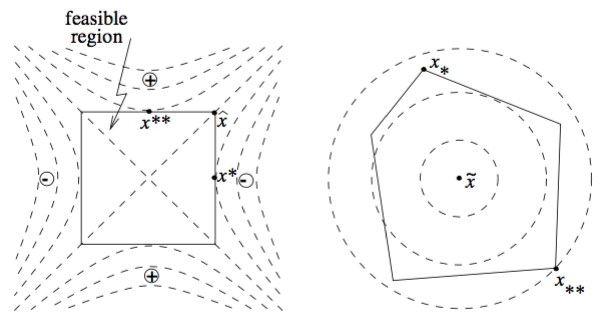
\includegraphics[scale=0.5]{Figures/Degeneracy_2.png}
			\decoRule
			\caption[hypercube]{Nonconvex quadratic programs.}
		\label{fig:Degeneracy_1}
	\end{figure}
	\begin{figure}[h]
		\centering
			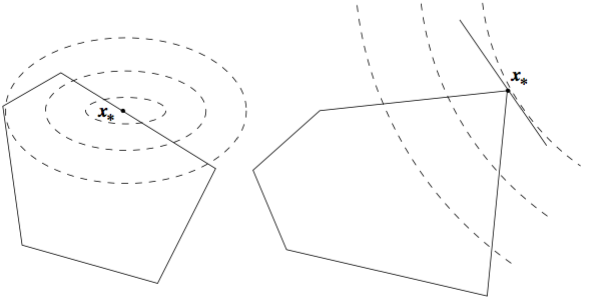
\includegraphics[scale=0.5]{Figures/Degeneracy_1.png}
			\decoRule
			\caption[hypercube]{Degenerate solutions of quadratic programs.}
		\label{fig:Degeneracy_2}
	\end{figure}
\end{itemize}
In the figure \ref{fig:Degeneracy_2} two instances are visualized. There is only a single active constraint at the solution $x^*$ in the left picture, that is lso an unconstrained minimizer of the objective function. According to KKT condition, $Gx^*+c=0$, such that the lone Lagrange multiplier should be zero.  3 constraints are active at the solution $x^*$ in the right-side image. As each of the three constraint gradients is a a vector in $\mathbb{R}^2$, they should be linearly independent.

Specifically for two reason Degeneracy can cause problems for optimization algorithms,
\begin{itemize}
	\item First linear dependence of the active constraint gradients can cause numerical difficulties as several matrices which required to factor become rank deficient.
	\item Second when the problem contains weakly active constraints, it is difficult for the algorithm to determine whether these constraints are active at the solution.
\end{itemize} 





\section{Active-set Methods for Convex QPs}
Active-set methods are important method for solving convex quadratic programs which consists equality and inequality constraints. Active set method starts by finding a feasible point during initial phase and then search for a solution along the edges and faces of the feasible set by solving a sequence of equality-constrained QPs.

If it was possible to know the contents of the active set earlier, it would be straight forward to get the solution by solving an equality-constrained QP of the form:
\begin{equation*}
	\begin{aligned}
		& \underset{x}{\text{min}} & & q(x)= \frac{1}{2}x^{T}Gx+x^{T}c \\
& \text{subject to} & &  a_{i}^{T}x = b_i & \forall i\in \mathcal{A}(x^*)
	\end{aligned}
\end{equation*}
But usually it is not possible to know $\mathcal{A}(x^*)$ and termination of this set is a major challnage for algorithms.

Primal active-set method follows step from one iteration to another by solving a quadratic subproblem in which some of the equality constraints and all the inequality constraints are imposed as equalities which is referred to as the working set. Working set at $k$th iterate $x_k$ is denoted by $\mathcal{W}_k$

Consider an iterate $x_k$ and the working set $\mathcal{W}_k$, it is necessary to check if $x_k$ minimizes the quadratic $q$ in the subspace defined by working set. Otherwise step p is computed by solving an equality-constrained subproblem in which the constraints corresponding to the working set $\mathcal{W}_k$ are regarded as equalities and all other constraints are temporarily disregarded. We define this subproblem in terms of the step p:
\begin{equation*}
	\begin{aligned}
		p = x - x_k, & & g_k = Gx_k + c.
	\end{aligned}
\end{equation*}

By substituting $x$ with $(x_k+p)$ into \ref{eqn:quadratic_programming},
\begin{equation*}
	\begin{aligned}
		q(x) = q(x_k+p)= \frac{1}{2}p^TGp+g_k^Tp+\rho_k
	\end{aligned}
\end{equation*}
$\rho_k$ is independent of p. So without considering $\rho_k$, we can write the QP subproblem to be solved at $k$th iteration as:

\begin{equation}
	\begin{aligned}
		& \underset{x}{\text{min}} & & \frac{1}{2}p^{T}Gp+g_{k}^{T}p \\
& \text{subject to} & &  a_{i}^{T}p = 0 & \forall i\in \mathcal{W}_k
	\end{aligned}
	\label{eqn:Active_set_1}
\end{equation}

Solution of this subproblem is denoted by $p_k$. Consider optimal $p_k$ is nonzero for the moment. We need to calculate displacement along this direction. If $x_k+p_k$ is feasible with respect to all the constraints, then we can set:
\begin{equation*}
\begin{aligned}
	x_{k+1} = x_k + p_k
\end{aligned}
\end{equation*} 
Otherwise, we set:
\begin{equation}
	\begin{aligned}
		x_{k+1} = x_k + \alpha_{k}p_{k}
	\end{aligned}
	\label{eqn:Active_set_2}
\end{equation}
Where $\alpha_k$ is the step length and is chosen possible largest value in the range $[0,1]$ for which all constraints are satisfied.

\subsection*{Selecting $\alpha_k$}
If $a_{i}^{T}p_{k} \geqslant 0$ for some $i\notin \mathcal{W}_k$, then for all $\alpha_k \geqslant 0$ we have $a_{i}^T(x_k+\alpha_kp_k)\geqslant a_{i}^Tx_k \geqslant b_i$. So, constraint $i$ will be satisfied for all nonnegative choices of the step-length parameter. Whenever $a_i^Tp_k < 0$ for some $i\notin \mathcal{W}_k$, we have  $a_{i}^T(x_k+\alpha_kp_k) \geqslant b_i$ only if
\begin{equation*}
	\begin{aligned}
		\alpha_k \leqslant \frac{b_i-a_i^Tx_k}{a_i^Tp_k}
	\end{aligned}
\end{equation*}
So, to maximize the decrement of q, $\alpha_k$ should be as large as possible in $[0,1]$ subject to retaining feasibility, so we get the following equation:

\begin{equation}
	\begin{aligned}
		\alpha_k = {\text{min}} \left( 1, \underset{i\notin \mathcal{W}_k,a_i^Tp_k<0 }{\text{min}} \frac{b_i-a_i^Tx_k}{a_i^Tp_k} \right) 
	\end{aligned}
	\label{eqn:Active_set_3}
\end{equation}

The constraints $i$ for which the minimum is achieved called blocking constraints. 

If $\alpha_k = 1$ and no new constraints are active at $ x_k+\alpha_kp_k $, then there is no blocking constraints on this iteration. 

If $\alpha_k < 1$, step along $p_k$ was blocked by some constraints not in $\mathcal{W}_k$, $\mathcal{W}_{k+1}$ is built by adding one of the blocking constraints to $\mathcal{W}_k$

This method is repeated untill a point $\hat{x}$ has been achieved that minimizes the quadratic objective function over its current working set $\hat{\mathcal{W}}$. Identifying this point is not hard because the subproblem as solution $p=0$. Since $p=0$ satisfies the optimality condition \ref{eqn:Properties_of_EC_QP_2} for \ref{eqn:Active_set_1}, it is found that:

\begin{equation}
	\begin{aligned}
		\underset{i\in \hat{\mathcal{W}}}{\sum}a_i\hat{\lambda}_i = g = G\hat{x}+c
	\end{aligned}
	\label{eqn:Active_set_4}
\end{equation}

for some Lagrange multipliers $\hat{\lambda}_i,i \in \hat{\mathcal{W}}$.  It follows that $x^*$ and $\lambda^*$ satisfy the first KKT condition, if the multipliers are defined corresponding to the inequality constraints that are not in the working set to be zero. As there are some control imposed on the step length, $x^*$ is also feasible with respect to all the constraints, so the second and third KKT conditions are satisfied at this point.\\

Considering the signs of the multipliers corresponding to the inequality constraints in the working set, that is, the indices $i\in \hat{\mathcal{W}} \cap \mathcal{I}$. The fourth KKT condition is also satisfied if these multipliers are all nonnegative. So it can be concluded that, $\hat{x}$ is a KKT point for the original problem \ref{eqn:quadratic_programming}. In fact, since G is positive semidefinite, we have from Theorem *** that $\hat{x}$ is a global solution of \ref{eqn:quadratic_programming}.

If on the other hand, if there exists some $j \in \hat{\mathcal{W}}\cap \mathcal{I}$, such that
\begin{equation*}
	\begin{aligned}
		\lambda^* < 0
	\end{aligned}
\end{equation*}

That constraints has to be removed from the active set and solve new subproblem. This will decreases the objective function. The following theorem states that this strategy produces a direction $p$ at the next iteration  that is feasible with respect to the removed constraint.
\begin{mybox}{Theorem}
\begin{theorem}
	Suppose that the point $\hat{x}$ satisfies first-order conditions for the equality-constrained subproblem with working set $\hat{W}$; that is, equation \ref{eqn:Active_set_3} is satisfied along with $a_i^T\hat{x}=b_i$ for all $i\in \hat{W}$ . Suppose, too, that the constraint gradients $a_i,i\in \hat{W}$, are linearly independent and that there is an index $j\in \hat{W}$ such that $\hat{lambda}_j<0$. 
	
	Let $p$ be the solution obtained by dropping the constraint $j$ and solving the following subproblem:
	\begin{equation}
	\begin{aligned}
		& \underset{p}{\text{min}} & & \frac{1}{2}p^{T}Gp+(G\hat{x}+c)^{T}p, \\
& \text{subject to} & &  a_{i}^{T}p = 0 & \forall i\in \hat{\mathcal{W}} \text{ with } i\neq j
	\end{aligned}
	\label{eqn:Active_set_5}
\end{equation}
Then $p$ is a feasible direction for constraint $j$,that is, $a_j^Tp \geqslant 0$. Moreover,if $p$ satisfies second- order sufficient conditions for above equation, then we have that $a_j^T > 0$, and that $p$ is a descent direction for $q(.)$.
\end{theorem}
\end{mybox}
Whenever $p_k$ obtained from \ref{eqn:Active_set_1} is nonzero and satisfies second-order sufficient optimality conditions for the current working set, it is a direction of strict descent for $q(.)$


\begin{mybox}{Theorem}
\begin{theorem}
	Suppose that the solution $p_k$ of \ref{eqn:Active_set_1} is nonzero and satisfies the second order sufficient conditions for optimality for that problem. Then the function $q(.)$ is strictly decreasing along the direction $p_k$ .
\end{theorem}
\end{mybox}

So it can be concluded that, When G is positive definite-the second order sufficient conditions are satisfied for all feasible subproblems of the form \ref{eqn:Active_set_1}. Hence, it follows from the result that a strict decrease in $q(.)$ can be obtained whenever $p_k \neq 0$.

\subsection*{Specification of the Active-set method for convex QP}
The whole Active-set algorithm can be specified as following:

\begin{algorithm}[h]
  \caption{Active-set method for convex QP}\label{euclid}
  \begin{algorithmic}[1]
    \Procedure{ActiveSet}{}
      \State Compute a feasible starting point $x_0$;
      \State Set $\mathcal{W}_0$ to be a subset of the active constraints at $x_0$;
      \For{\texttt{$k=0,1,2,...$}}
        \State Solve \ref{eqn:Active_set_1} to find $p_k$;
        \If{$p_k==0$}
          \State Compute Lagrange multipliers $\hat{\lambda}$ that satisfy \ref{eqn:Active_set_1} with $\hat{\mathcal{W}}==\mathcal{W}_k$
          \If{$\hat{\lambda} \geqslant 0$} for all $i \in \mathcal{W}\cap \mathcal{I}$
          	\State Stop with solution $x^* = x_k$
          \Else
          	\State $j \gets argmin_{j\in \mathcal{W}_k \cap \mathcal{I}}$ $\hat{\lambda}_j$
          	\State $x_{k+1} \gets x_k$
          	\State $\mathcal{W}_{k+1} \gets \mathcal{W}_k\backslash \lbrace{j \rbrace}$
          \EndIf 
        \Else
          \State $\alpha_k$ from \ref{eqn:Active_set_3}
          \State $x_{k+1} \gets x_k + \alpha_kp_k$
          \If{there are blocking constraints}
          	\State obtain $\mathcal{W}_{k+1}$ by adding one of the blocking constraints to $\mathcal{W}_k$
          \Else
          	\State $\mathcal{W}_{k+1} \gets \mathcal{W}_k$  
          \EndIf
        \EndIf
      \EndFor
    \EndProcedure
  \end{algorithmic}
\end{algorithm}
To implement active-set method efficiently an important key is reuse of nformation from solving the equality-constrained subproblem at the next iteration. The only difference between two consecutive subproblems is that the working set grows or shrinks by a single component. Efficient codes perform updates of the matrix factorizations obtained at the previous iteration, rather than calculating them from scratch each time.



\section{Interior-Point Method}
Interior-point methods follow iterative approach which is a good candidate as alternative of active-set method. This method is also know as trajectory-following, path-following method. 
Here only convex quadratic programming problem with inequality constraints will be focused. It is easier to the problem as follows:

\begin{equation}
\begin{aligned}
& \underset{x}{\text{min}}
& & q(x)= \frac{1}{2}x^{T}Gx+x^{T}c \\
& \text{subject to} & &  Ax \geqslant b
\end{aligned}
\label{eqn:Path_following_1}
\end{equation}

where $G\in \mathbb{R}^{n\times n}$ is symmetric, positive semidefinite, $A\in \mathbb{R}^{m\times n}$.
\begin{equation*}
	\begin{aligned}
		A = [a_i]_{i\in \mathcal{I}} & & b = [b_i]_{i\in \mathcal{I}}, & & \mathcal{I}=\lbrace 1,2,3...,m \rbrace 
	\end{aligned}
\end{equation*}

KKT conditions for this notation can be written as follows:
\begin{equation}
	\begin{aligned}
		Gx- A^T\lambda + c &= 0,\\
		Ax - b  &\geqslant 0, \\
		(Ax-b)_i\lambda_i &= 0, & & i = 1,2,...,m\\
		\lambda &\geqslant 0.
	\end{aligned}
	\label{eqn:Path_following_2}
\end{equation}
By introducing the slack vector $y \geqslant 0$, conditions can be rewritten as:
\begin{equation}
	\begin{aligned}
		Gx- A^T\lambda + c &= 0,\\
		Ax - y - b  &= 0, \\
		y_i\lambda_i &= 0, & & i=1,2,...,m\\
		(y,\lambda) \geqslant 0,
	\end{aligned}
	\label{eqn:Path_following_3}
\end{equation}

As $G$ is positive semidefinite, above KKT conditions are necessary and sufficient to solve convex quadratic program.

Let, current iterate $(x,y,z)$ that satisfies $(y,\lambda)>0$, a complementary measure $\mu$ can be defined as:
\begin{equation}
	\begin{aligned}
		\mu = \frac{y^T\lambda}{m}
	\end{aligned}
	\label{eqn:Path_following_4}
\end{equation}
Derived path-following for the KKT conditions by considering the above KKT conditions:

\begin{equation}
\begin{aligned}
F(x,y,\lambda:\sigma,\mu) = 
\begin{bmatrix}
  	Gx-A^T\lambda+c\\
    Ax-y-b\\
    \mathcal{Y} \Lambda e - \sigma \mu e
  \end{bmatrix}
  =0
\end{aligned}
\label{eqn:Path_following_5}
\end{equation}

Where
\begin{equation*}
	\begin{aligned}
		\mathcal{Y} = diag(y_1,y_2,...,y_m), & & \Lambda = diag(\lambda_1 , \lambda_2,...,\lambda_1), & & e = (1,1,...,1)^T
	\end{aligned}
\end{equation*}
and  $\sigma \in [0,1]$. The solution of \ref{eqn:Active_set_5} for all positive values of $\sigma$ and $\mu$ define the central path, which is a trajectory that leads to the solution to the QP as $\sigma \mu$ tends to zero.

After selecting $\mu$ and applying Newton's method to \ref{eqn:Active_set_5} the following linear system is achieved:
\begin{equation}
	\begin{aligned}
		\begin{bmatrix}
			G & 0 & -A^T\\
			A & -I & 0\\
			0 & \Lambda & \mathcal{Y} 
		\end{bmatrix}
		\begin{bmatrix}
			\Delta x\\
			\Delta y\\
			\Delta \lambda
		\end{bmatrix}
		=
		\begin{bmatrix}
			-r_d\\
			-r_p\\
			-\Lambda \mathcal{Y}e + \sigma \mu e
		\end{bmatrix}
	\end{aligned}
	\label{eqn: Path_planning_6}
\end{equation}

where
\begin{equation*}
	\begin{aligned}
		r_d = Gx-A^T\lambda +c & & r_p = Ax-y-b
	\end{aligned}
\end{equation*}

The new iterate $(x^+,y^+,\lambda^+)$ are obtained by means of
\begin{equation*}
	\begin{aligned}
		(x^+,y^+,\lambda^+) = (x,y,\lambda) + \alpha (\Delta x, \Delta y, \Delta \lambda )
	\end{aligned}
\end{equation*}

$\alpha$ is chosen such that $(x^+,\lambda^+)>0$ and possibly to satisfy various other conditions.












































